\documentclass[conference]{IEEEtran}
\IEEEoverridecommandlockouts
% The preceding line is only needed to identify funding in the first footnote. If that is unneeded, please comment it out.
\usepackage{cite}
\usepackage{amsmath,amssymb,amsfonts}
\usepackage{algorithmic}
\usepackage{graphicx}
\graphicspath{{../../results/paper_full/plots/}}
\usepackage{textcomp}
\usepackage{microtype}
\usepackage{xcolor}
\def\BibTeX{{\rm B\kern-.05em{\sc i\kern-.025em b}\kern-.08em
    T\kern-.1667em\lower.7ex\hbox{E}\kern-.125emX}}
\usepackage{tikz}
\usetikzlibrary{arrows.meta,positioning,shapes.geometric,fit,calc}
\usepackage{pgfplots}
\pgfplotsset{compat=1.18}
\emergencystretch=2em
\raggedbottom
\begin{document}

\title{RAPID-Learn: A Resource-Aware Lightweight Adaptive Learning Framework for Low-Resource Environments}

\author{
\IEEEauthorblockN{Kapil Jangid}
\IEEEauthorblockA{\textit{Department of Computer Engineering} \\
\textit{Silver Oak University}\\
Ahmedabad, India \\
kapil31jangid@gmail.com}
\and
\IEEEauthorblockN{2\textsuperscript{nd} Given Name Surname}
\IEEEauthorblockA{\textit{dept. name of organization (of Aff.)} \\
\textit{name of organization (of Aff.)}\\
City, Country \\
email address or ORCID}
}

\maketitle

\begin{abstract}
Adaptive learning systems often assume computational resources and connectivity that are unavailable in low-resource educational settings. This paper presents RAPID-Learn (Resource-Aware, Personalised and Intelligent Dynamic Learning), a lightweight, explainable, and offline-capable framework combining Bayesian Knowledge Tracing, independent uncertainty, retained mastery, prerequisite and misconception reasoning, resource-aware control, metadata-driven activity ranking, and an optional logistic-regression predictor with complete fallback to BKT. We evaluate the implemented system using 900,000 synthetic interactions from nine runtime conditions, 500 learners per condition and seed, 40 interactions per learner, and five seeds. Full RAPID-Learn achieved response accuracy of 0.5569 versus 0.5108 for Static and synthetic retention of 0.9619 versus 0.9222, but its synthetic normalized gain was lower (0.1523 versus 0.3034). Misconception handling produced the clearest positive ablation effect: Full-minus-No-Misconceptions accuracy was $+0.0804$ (95\% CI $[+0.0772,+0.0825]$), with normalized-gain difference $+0.0064$ ($[+0.0049,+0.0082]$). Resource-awareness gain and utility intervals included zero, and the optional predictor showed poor synthetic probability quality and no established incremental benefit. Tested resource- and activity-weight perturbations did not reverse the principal findings. These simulation results demonstrate reproducible controller behaviour and expose important trade-offs; they do not establish classroom effectiveness or general educational superiority.
\end{abstract}

\begin{IEEEkeywords}
adaptive learning, Bayesian Knowledge Tracing, resource-aware computing, personalized learning, offline learning, lightweight artificial intelligence, low-resource environments
\end{IEEEkeywords}

\section{Introduction}

Artificial Intelligence (AI) has increasingly influenced digital education by enabling learning systems to respond to differences in learner knowledge, performance, pace, and interaction behaviour. Conventional digital learning platforms commonly present similar instructional sequences to learners despite substantial variation in prior knowledge and learning requirements. Adaptive learning seeks to address this limitation by continuously estimating learner state and modifying instructional content, difficulty, feedback, or progression according to individual needs \cite{mittal2024,tan2025}. Machine learning, knowledge-tracing techniques, reinforcement learning, natural language processing, and generative AI have consequently been investigated for learner modelling, performance prediction, recommendation, adaptive assessment, and intelligent tutoring \cite{hariyanto2025,ruan2025}.

The effectiveness of an adaptive learning system depends on its ability to maintain an informative learner representation and translate that representation into pedagogically appropriate decisions. Typical adaptive architectures incorporate a learner model describing current knowledge and interaction history, a domain model representing concepts and prerequisite relationships, and an adaptation mechanism responsible for selecting subsequent instructional activities \cite{tan2025,pelanek2024rules}. Learner interactions such as response correctness, attempts, response time, progression, and recent performance can therefore be used to estimate mastery and determine whether a learner should progress, review previous material, receive remediation, or attempt a different activity.

Several studies have demonstrated the potential of adaptive learning to improve personalization, learner engagement, feedback, and academic performance \cite{contrino2024,merino2025}. However, increasingly sophisticated personalization techniques also introduce practical deployment challenges. Deep neural architectures, reinforcement-learning systems, multimodal learner models, and large language models can require substantial computational resources, extensive training data, continuous connectivity, or remote cloud services. These assumptions may be reasonable in well-resourced environments but are considerably harder to satisfy in rural schools, community learning centres, low-income institutions, and educational environments where learners depend on low-cost devices and intermittent connectivity \cite{pelanek2025hard,amin2023}.

Resource constraints in such environments extend beyond computational performance. Limited memory and processing capacity can restrict the models that can be executed locally, while unreliable connectivity can prevent access to cloud-hosted learning resources. Device battery availability, storage limitations, and network conditions can further affect whether an otherwise pedagogically suitable activity can be delivered effectively. Consequently, an adaptive system intended for low-resource deployment should consider not only what a learner needs pedagogically, but also what the learner's current device and connectivity conditions can support.

Another important challenge is interpretability. Adaptive decisions directly influence the instructional material presented to a learner, including progression, remediation, review, and difficulty adjustment. Educators should therefore be able to determine why a particular recommendation was generated. Rule-based and modular recommendation approaches provide transparency because their decision logic can be explicitly inspected \cite{pelanek2024rules}. However, purely deterministic rules may be insufficient for representing uncertainty in learner knowledge or predicting response behaviour from interaction history. Conversely, complex predictive models can capture behavioural patterns but may reduce interpretability and increase computational cost.

Knowledge tracing provides an intermediate approach for maintaining learner state without requiring large computational models. Bayesian Knowledge Tracing (BKT), in particular, represents learner mastery probabilistically and updates the estimated probability of knowledge as evidence is observed. Nevertheless, mastery alone may not capture every instructional consideration. A learner may exhibit uncertain performance, retain previously mastered concepts imperfectly over time, repeatedly demonstrate a specific misconception, or be blocked by unmet prerequisites. These signals can affect the appropriate instructional decision even when estimated mastery values are similar.

This work therefore investigates adaptive learning as a joint pedagogical and resource-allocation problem. Rather than selecting activities solely from estimated learner performance, an adaptive controller should consider multiple forms of evidence including current mastery, uncertainty, knowledge retention, prerequisite satisfaction, misconceptions, learning history, availability of offline content, and computational resource conditions.

To address these requirements, this paper presents RAPID-Learn (Resource-Aware, Personalised and Intelligent Dynamic Learning), a lightweight adaptive learning framework designed for resource-constrained educational environments. RAPID-Learn combines Bayesian Knowledge Tracing with independent learner-uncertainty estimation, retained-mastery modelling, prerequisite reasoning, misconception detection, resource monitoring, and an explainable deterministic controller. The framework additionally supports an optional lightweight machine-learning predictor for candidate-level response estimation. When the predictive artefact is missing, incompatible, or fails validation, the recommendation pipeline safely falls back to the BKT-based mechanism rather than interrupting adaptation.

The learner model maintains concept-specific mastery and interaction history while treating uncertainty as a separate signal. Retained mastery is derived using a time-dependent forgetting mechanism, allowing previously learned concepts to become candidates for spaced review when estimated retention decreases. Curriculum concepts are represented through an explicit prerequisite graph, enabling the system to prevent inappropriate progression and recommend prerequisite review when necessary. Misconception evidence is accumulated from repeated recent incorrect responses and can trigger targeted remediation when sufficient evidence is available.

RAPID-Learn also incorporates resource conditions directly into adaptive decision-making. The resource monitor observes available memory, processor availability, network status, storage, and battery information when supported by the execution environment. These signals are summarized into a resource state that influences the controller and activity-ranking process. This design allows an activity with strong pedagogical relevance but excessive computational or connectivity requirements to be deprioritized when a more feasible alternative is available.

The recommendation mechanism evaluates candidate learning activities using pedagogical and computational criteria. Candidate ranking considers expected learning gain, prerequisite relevance, retention need, information gain, misconception relevance, and resource-adjusted computational cost. Explicit controller rules determine the adaptation pathway, while candidate ranking selects an appropriate activity within that pathway. This separation maintains explainability because the reason for an adaptive action can be recorded independently from the ranking process.

Offline operation is treated as a primary design requirement rather than an auxiliary feature. RAPID-Learn employs a progressive web application in which successfully retrieved instructional activities can be cached locally. During connectivity loss, available learning content can continue to be rendered from the local cache and learner interactions can be queued for later synchronization. Importantly, application-shell availability is distinguished from actual educational-content availability, preventing the system from assuming that a learning activity is accessible offline merely because the user interface has been cached.

The implemented prototype currently provides versioned curriculum pathways with original adaptive instructional materials aligned to Class 5 and Class 6 Mathematics topics. Learner state, curriculum metadata, interactions, mastery history, recommendations, controller explanations, and fallback information are persisted locally. The architecture separates curriculum representation, learner state, recommendation logic, resource monitoring, and application delivery to facilitate reproducibility and component-level evaluation.

A reproducible synthetic experimentation framework is used to study the behaviour of RAPID-Learn before classroom deployment. Synthetic learner state is maintained separately from the system's estimated mastery, preventing the adaptive controller from directly accessing the simulator's latent ground truth. The experimental framework supports multiple learner profiles, resource conditions, random seeds, baselines, and component ablations. Educational measures derived from simulation include response accuracy, mastery gain, normalized gain, retention, and time to mastery, while system-level measures include latency, memory usage, processor utilization, bandwidth consumption, and resource-normalized utility.

The synthetic evaluation is intended to determine whether the proposed controller retains useful adaptive behaviour under constrained computational conditions and to isolate the contribution of individual components. It does not constitute evidence of real-world educational effectiveness. Validation with actual learners remains necessary before claims regarding academic achievement or classroom learning outcomes can be established.

The main contributions of this work are summarized as follows:

\begin{itemize}

    \item An explainable, resource-aware adaptive learning architecture integrating Bayesian Knowledge Tracing, learner uncertainty, retained mastery, prerequisite reasoning, misconception evidence, and device-resource conditions.

    \item A hybrid adaptive decision mechanism that separates pedagogical pathway selection from candidate activity ranking while retaining auditable explanations for generated recommendations.

    \item A resource-aware recommendation strategy that incorporates pedagogical utility together with computational cost and offline-content availability.

    \item An offline-capable learning architecture that supports locally cached instructional activities and delayed synchronization of learner interactions under intermittent connectivity.

    \item An optional lightweight response-prediction mechanism with artifact validation and safe fallback to BKT, preventing dependence on machine-learning inference for basic adaptive functionality.

    \item A reproducible synthetic evaluation framework supporting baselines, multi-component ablations, independent simulator ground truth, multi-seed experimentation, bootstrap confidence intervals, and computational-efficiency measurements.

\end{itemize}

The remainder of this paper is organized as follows. Section II reviews previous work on adaptive learning, learner modelling, knowledge tracing, personalized recommendation, and resource-constrained educational technology. Section III presents the architecture and learner-modelling mechanisms of RAPID-Learn. Section IV describes the resource-aware adaptive controller and activity-recommendation strategy. Section V presents the experimental methodology, baselines, ablations, and evaluation metrics. Section VI reports the synthetic experimental results. Section VII discusses the findings, limitations, and threats to validity. Finally, Section VIII concludes the paper and outlines directions for classroom validation and future development.

\section{Related Work}

\subsection{AI-Driven Adaptive Learning}

Artificial Intelligence (AI)-enabled adaptive learning has evolved from
fixed instructional sequencing toward systems capable of estimating
learner state and dynamically modifying content, difficulty, feedback,
and learning pathways. Reviews of adaptive-learning platforms show that
learner models, domain models, and adaptation models form the principal
architectural components of these systems \cite{tan2025}. AI techniques
used within such environments include supervised learning, unsupervised
learning, reinforcement learning, knowledge tracing, multimodal
analytics, natural language processing, and generative AI
\cite{hariyanto2025,matos2025}.

Evidence from systematic and scoping reviews suggests that personalized
adaptive learning can improve academic performance, engagement,
feedback, and learning satisfaction, although reported effects vary
across technologies and educational contexts
\cite{merino2025,duplooy2024}. Contrino \textit{et al.}, for example,
reported improved achievement when adaptive learning was integrated
into both online and face-to-face university courses
\cite{contrino2024}. Similarly, controlled studies of machine-learning
and deep-learning personalization have reported improvements in
performance and engagement \cite{hassanain2025,naseer2024}.

However, increasingly sophisticated AI methods frequently assume access
to substantial computational resources, large datasets, or cloud
services. Deep reinforcement learning, multimodal architectures, and
large language models can provide advanced personalization but introduce
greater processing, data, infrastructure, and interpretability
requirements \cite{ruan2025,farhah2025,pereira2025}. This creates a
significant gap between personalization capability and practical
deployability in resource-constrained learning environments.

\subsection{Learner Modelling and Knowledge Tracing}

Learner modelling provides the state representation required for
adaptive instructional decisions. Common learner indicators include
response correctness, assessment performance, number of attempts,
response time, interaction history, completion behaviour, and prior
knowledge \cite{tan2025,duplooy2024}. Such indicators are attractive for
lightweight systems because they can usually be collected without
specialized sensors or high-dimensional multimodal data.

Bayesian Knowledge Tracing (BKT) remains a useful probabilistic approach
for representing concept mastery over time. Pelánek emphasizes that the
effectiveness of student modelling depends not only on predictive
accuracy but also on knowledge-component definition, granularity,
observational evidence, mastery criteria, and the instructional use of
the resulting estimates \cite{pelanek2025hard}. These trade-offs are
particularly relevant to low-resource systems where unnecessarily
complex learner models may increase computational cost without providing
proportional pedagogical benefit.

Existing research also suggests that mastery alone may be an incomplete
representation of learner state. Adaptive systems can benefit from
considering prior knowledge, confidence, self-regulation, preferences,
and contextual learner information \cite{dai2024,fujii2024,jin2023}.
Mejeh and Rehm further demonstrated that contextual information extracted
from learners can improve personalization, although their NLP-based
approach also introduces additional processing requirements
\cite{mejehrehm2024}. These findings motivate the use of multiple compact
learner indicators while avoiding dependence on computationally
expensive representations.

\subsection{Personalized Learning-Activity Recommendation}

Educational recommendation differs from conventional recommender systems
because activity selection must satisfy pedagogical constraints such as
mastery, prerequisites, progression, repetition, and curriculum
structure. Reviews of personalized educational recommendation identify
content-based, collaborative, hybrid, and data-driven approaches, while
also reporting challenges related to infrastructure, context awareness,
language, and scalability \cite{dhananjaya2024}.

Pelánek, Effenberger, and Jarušek proposed a modular rule-based approach
in which explicit IF--THEN rules consider mastery, prerequisite
relationships, difficulty, previous performance, interests, and spaced
practice \cite{pelanek2024rules}. The approach is particularly relevant
to interpretable educational systems because each recommendation can be
associated with a transparent reason and individual rules can be
modified independently.

Large-scale learner studies additionally indicate that recommendation
preferences may differ according to confidence, personality, subject,
and learner characteristics \cite{dai2024}. Adaptive educational search
has also demonstrated strong retrieval and personalization performance,
although such architectures typically assume online access and multiple
computational components \cite{li2025}. These findings support a hybrid
recommendation strategy that combines pedagogically explicit constraints
with lightweight data-driven evidence.

\subsection{Machine Learning and Reinforcement Learning for Adaptation}

Machine-learning techniques have been widely applied to learner
classification, performance prediction, adaptive sequencing, and course
customization. Hassanain \textit{et al.} reported improved performance,
engagement, and satisfaction in a controlled study using ML-based
personalization \cite{hassanain2025}. Deep-learning-based adaptive
pathways have similarly reported substantial improvements in university
learning contexts \cite{naseer2024}.

Reinforcement learning formulates adaptive sequencing as a sequential
decision-making problem. Amin \textit{et al.} used Q-learning and a
Markov Decision Process to model personalized sequential recommendation,
demonstrating the ability to react to changing learner behaviour
\cite{amin2023}. More recent work has extended this direction through
deep reinforcement learning and multimodal learner information
\cite{ruan2025}.

Despite their personalization capability, these approaches introduce
challenges involving state-space complexity, cold-start behaviour,
reward design, training requirements, data sparsity, and
interpretability \cite{amin2023,ruan2025}. RAPID-Learn therefore treats
machine-learning prediction as a complementary mechanism rather than as
a mandatory dependency of adaptive operation.

\subsection{Uncertainty, Forgetting, and Misconceptions}

Effective adaptation requires distinguishing different causes of weak
learner performance. A learner may have low mastery, insufficient
evidence for a reliable mastery estimate, forgotten previously mastered
content, failed a prerequisite, or developed a persistent
misconception. Treating these situations identically can result in
inappropriate recommendations.

Pelánek highlights uncertainty, mastery estimation, model granularity,
and observational limitations as fundamental challenges in adaptive
learner modelling \cite{pelanek2025hard}. Research on adaptive
recommendation also supports the use of spaced repetition and
prerequisite relationships when determining subsequent activities
\cite{pelanek2024rules}. Learning-analytics systems further demonstrate
the value of explicitly identifying misconceptions and learning
progression when supporting personalized interventions
\cite{sajja2025}.

These findings motivate RAPID-Learn's separation of mastery,
uncertainty, retained mastery, prerequisite readiness, and misconception
evidence. Rather than encoding all learner conditions within a single
prediction score, each signal contributes independently to the adaptive
decision process.

\subsection{Resource-Constrained and Offline Learning}

Infrastructure remains a major barrier to equitable AI-supported
education. Systematic reviews identify computational cost, connectivity,
privacy, digital access, scalability, and unequal infrastructure as
continuing challenges for personalized AI systems
\cite{hariyanto2025,mimoudi2025}. Teachers working in an open
distance-learning context similarly reported unequal internet access,
limited AI knowledge, language barriers, and insufficient technological
resources as significant adoption constraints
\cite{vandenberg2025}.

Existing Education 4.0 architectures frequently depend on technologies
such as edge computing, IoT, 5G, augmented reality, and remote
laboratories \cite{boltsi2024}. While such technologies provide advanced
learning capabilities, their infrastructure assumptions may not be
appropriate for institutions operating with inexpensive devices and
intermittent networks.

Sustainability-oriented adaptive-learning research has begun to
recognize computational efficiency as a design consideration.
Ezzaim \textit{et al.} proposed a multi-factor adaptive architecture
incorporating resource optimization and Green AI principles
\cite{ezzaim2024}. However, the architecture was not empirically
validated under low-resource deployment conditions. This leaves an
opportunity for adaptive systems in which computational-resource
conditions participate directly in recommendation rather than being
treated only as implementation constraints.

Offline learning introduces an additional requirement. Educational
content must be locally accessible, learner interactions must survive
connectivity loss, and adaptive functionality should not depend entirely
on remote inference. These requirements motivate the explicit treatment
of offline-content availability and device conditions within
RAPID-Learn.

\subsection{Generative AI and Human Oversight}

Generative AI has expanded opportunities for personalized explanations,
feedback, tutoring, assessment, and adaptive curriculum generation
\cite{mittal2024,pereira2025}. Controlled experiments have shown that
context-personalized AI-generated learning material can improve
motivation and performance \cite{tasdelen2025}. A recent randomized
study also reported stronger performance and engagement from a
GPT-4o-driven adaptive curriculum than from a static curriculum
\cite{samat2026}.

However, these benefits are accompanied by concerns involving
hallucination, bias, privacy, infrastructure dependency, unequal access,
and reliance on commercial cloud APIs
\cite{mittal2024,mimoudi2025}. Studies comparing AI-generated and
teacher-generated explanations further indicate that AI content is not
uniformly preferable across concepts \cite{lee2024}.

Human oversight therefore remains important. Studies of human--AI
collaboration suggest that educators and AI systems provide
complementary capabilities, particularly for contextual judgement,
feedback, and instructional moderation
\cite{tzirides2024,pahi2024}. Co-design research also demonstrates that
teacher and learner participation can improve the usability and
pedagogical alignment of adaptive technology
\cite{mejeh2025codesign}. These findings support RAPID-Learn's
interpretable controller and teacher-supervised adaptation approach.

\subsection{Hybrid and Explainable Adaptive Learning}

Hybrid systems provide an opportunity to combine transparent
pedagogical reasoning with data-driven learner evidence. Rule-based
recommendation offers interpretability and modularity
\cite{pelanek2024rules}, while machine-learning approaches can discover
patterns that cannot easily be encoded through manually specified
conditions \cite{hassanain2025}.

Practical educational systems have already combined learner profiles,
adaptive pathways, conversational interfaces, and AI-based feedback.
Chen \textit{et al.}, for example, developed an adaptive educational
chatbot supporting self-assessment, topic recommendation, and customized
feedback \cite{chen2025}. However, its dependence on cloud-based
services and large-language-model support limits direct applicability to
resource-constrained offline environments.

Explainability is also increasingly recognized as an educational and
governance requirement. International expert research identifies
trustworthiness, privacy, fairness, equity, and understandable AI
decision-making as important priorities for educational AI
\cite{ifenthaler2024}. A lightweight hybrid controller can therefore be
advantageous when adaptive recommendations must remain auditable by
teachers and administrators.

\subsection{Research Gap}

The reviewed literature demonstrates substantial progress in adaptive
learning, learner modelling, recommender systems, reinforcement learning,
generative AI, and human--AI educational interaction. Nevertheless, four
limitations remain particularly relevant to low-resource deployment.

First, sophisticated adaptive approaches often optimize predictive or
recommendation performance while assuming reliable computational
infrastructure and connectivity
\cite{ruan2025,naseer2024,samat2026}. Second, resource limitations are
commonly discussed as deployment barriers rather than incorporated
directly into adaptive decision-making
\cite{hariyanto2025,mimoudi2025,ezzaim2024}. Third, learner state is
often represented primarily through performance or mastery even though
uncertainty, forgetting, prerequisites, and misconceptions can require
different instructional responses \cite{pelanek2025hard,pelanek2024rules}.
Finally, highly data-driven approaches can reduce interpretability,
whereas purely rule-based systems may not exploit useful patterns in
learner interactions.

RAPID-Learn addresses these limitations through an integrated
resource-aware architecture combining Bayesian Knowledge Tracing,
independent uncertainty estimation, retained mastery, prerequisite
reasoning, misconception evidence, device-resource monitoring,
offline-content availability, and explainable adaptive control. An
optional lightweight predictor augments this architecture without
becoming a mandatory dependency. The resulting design targets a balance
among personalization, interpretability, computational efficiency, and
connectivity resilience.

\section{RAPID-Learn System Architecture}

RAPID-Learn is designed as a modular adaptive learning architecture in which learner modelling, curriculum representation, adaptive decision-making, resource monitoring, recommendation, and content delivery remain logically separated. This separation enables individual components to be inspected, modified, and evaluated independently while preserving a common interaction pipeline.

The implemented prototype uses a FastAPI backend with local SQLite persistence and a React-based progressive web application (PWA). Curriculum metadata and learner-facing instructional activities are represented using versioned structured data. The current prototype includes original adaptive instructional resources aligned to Class 5 and Class 6 Mathematics pathways.

\begin{figure*}[t]
\centering

\resizebox{0.95\textwidth}{!}{
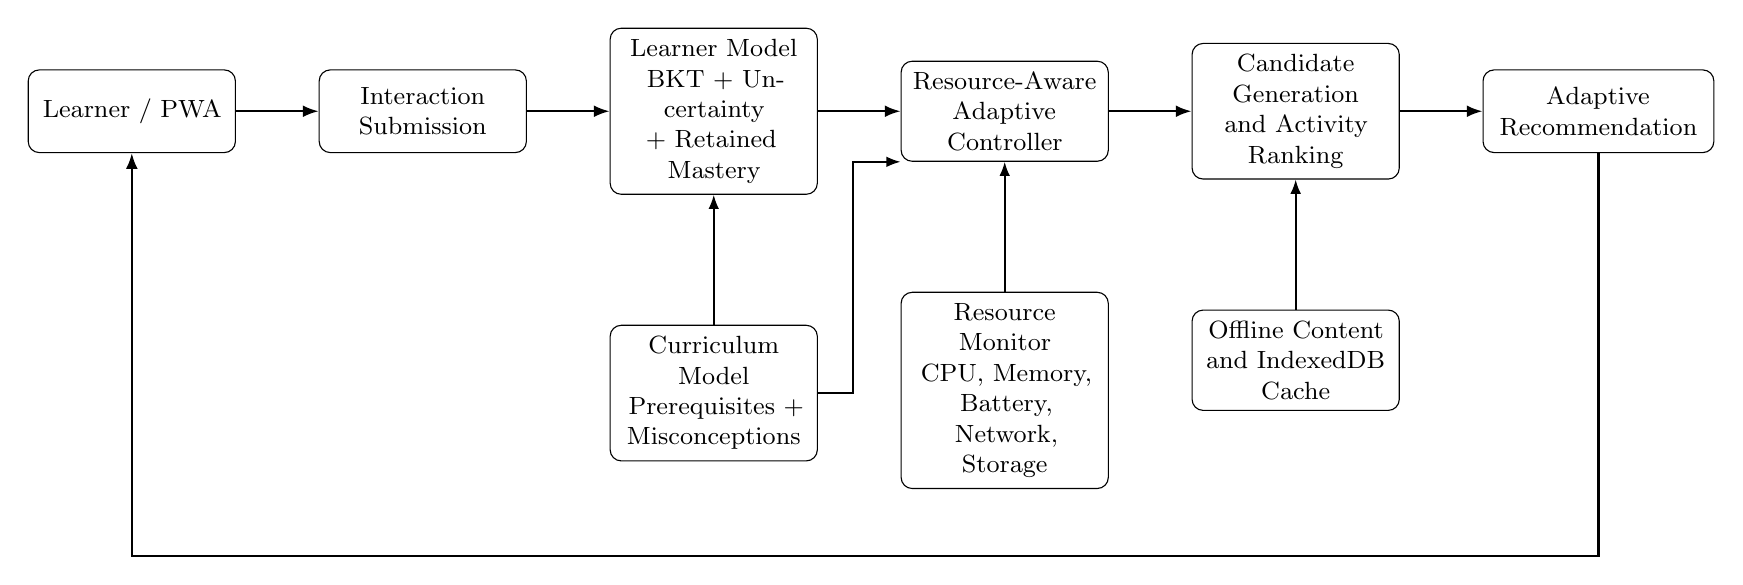
\begin{tikzpicture}[
    node distance=1.1cm and 1.05cm,
    mainbox/.style={
        rectangle,
        rounded corners,
        draw,
        align=center,
        text width=2.35cm,
        minimum height=1.05cm,
        inner sep=4pt,
        font=\small
    },
    supportbox/.style={
        rectangle,
        rounded corners,
        draw,
        align=center,
        text width=2.35cm,
        minimum height=1.15cm,
        inner sep=4pt,
        font=\small
    },
    arrow/.style={
        -{Latex[length=2mm]},
        thick
    },
    supportarrow/.style={
        -{Latex[length=1.8mm]},
        semithick
    }
]

% =========================
% Top pipeline
% =========================

\node[mainbox] (learner)
{Learner / PWA};

\node[mainbox, right=of learner] (interaction)
{Interaction\\Submission};

\node[mainbox, right=of interaction] (model)
{Learner Model\\BKT + Uncertainty\\+ Retained Mastery};

\node[mainbox, right=of model] (controller)
{Resource-Aware\\Adaptive Controller};

\node[mainbox, right=of controller] (ranker)
{Candidate Generation\\and Activity Ranking};

\node[mainbox, text width=2.65cm, right=of ranker] (recommendation)
{Adaptive\\Recommendation};

% =========================
% Supporting layer
% =========================

\node[supportbox, below=1.65cm of model] (domain)
{Curriculum Model\\Prerequisites +\\Misconceptions};

\node[supportbox, below=1.65cm of controller] (resource)
{Resource Monitor\\CPU, Memory, Battery,\\Network, Storage};

\node[supportbox, below=1.65cm of ranker] (offline)
{Offline Content\\and IndexedDB Cache};

% =========================
% Main forward flow
% =========================

\draw[arrow] (learner.east) -- (interaction.west);
\draw[arrow] (interaction.east) -- (model.west);
\draw[arrow] (model.east) -- (controller.west);
\draw[arrow] (controller.east) -- (ranker.west);
\draw[arrow] (ranker.east) -- (recommendation.west);

% =========================
% Support connections
% =========================

\draw[supportarrow] (domain.north) -- (model.south);

\draw[supportarrow]
(domain.east)
-- ++(0.45,0)
|- (controller.south west);

\draw[supportarrow]
(resource.north)
-- (controller.south);

\draw[supportarrow]
(offline.north)
-- (ranker.south);

% =========================
% Clean feedback loop
% =========================

\coordinate (feedbackY) at ($(resource.south)+(0,-0.85)$);

\draw[arrow]
(recommendation.south)
-- ++(0,-2.05)
|- (feedbackY)
-| (learner.south);

\end{tikzpicture}
}

\caption{Architecture of RAPID-Learn showing learner-state estimation, resource-aware adaptation, activity ranking, and offline feedback flow.}
\label{fig:rapid_architecture}
\end{figure*}

\subsection{Design Objectives}

RAPID-Learn is guided by five primary design objectives:

\begin{enumerate}
    \item \textbf{Personalization:} instructional activities should respond to individual learner state rather than follow a fixed sequence.

    \item \textbf{Computational Efficiency:} core adaptation should remain feasible on resource-constrained devices without dependence on computationally intensive models.

    \item \textbf{Interpretability:} adaptive decisions should expose the pedagogical evidence and controller rule responsible for the selected pathway.

    \item \textbf{Connectivity Resilience:} essential learning and adaptation functionality should remain available when network connectivity is intermittent.

    \item \textbf{Modularity:} knowledge tracing, misconception handling, resource awareness, optional machine learning, and recommendation should be independently configurable and ablatable.
\end{enumerate}

These objectives motivate an architecture in which learner state and pedagogical reasoning remain operational even when optional predictive or network-dependent components are unavailable.

\subsection{Curriculum and Domain Model}

The curriculum hierarchy in RAPID-Learn is represented as

\begin{equation*}
\begin{aligned}
\text{Board} &\to \text{Class} \to \text{Subject} \to \text{Book}\\
             &\to \text{Chapter} \to \text{Concept}.
\end{aligned}
\end{equation*}

Each concept can be associated with learning activities, assessment questions, difficulty information, prerequisite relationships, and misconception metadata. Stable concept and activity identifiers are used so that learner progress remains associated with the appropriate curriculum element even when instructional pathways change.

Prerequisite relationships form a directed graph. A concept becomes normally eligible for progression only when its direct prerequisites satisfy their corresponding mastery thresholds. The graph can also support explicit prerequisite-review recommendations when a learner requires reinforcement from an earlier concept or class.

Learning activities form the primary recommendation objects. Activity metadata describes supported adaptation pathways, difficulty, availability for offline use, bundled-content status, estimated computational cost, misconception links, and lifecycle state. Deprecated or inactive activities remain readable for historical records but are excluded from future recommendation generation.

\subsection{Learner Model}

RAPID-Learn maintains a separate learner state for each concept rather than representing performance through a single global score. Each interaction can contribute information including correctness, response time, previous attempts, concept history, and recent learner performance.

The central mastery estimator uses Bayesian Knowledge Tracing (BKT). Let $K_t$ denote whether a learner has mastered a concept at interaction $t$. BKT maintains the posterior mastery probability

\[
P(K_t \mid O_{1:t}),
\]

where $O_{1:t}$ represents the sequence of observed learner responses.

For a correct response, the posterior before learning transition can be expressed as

\begin{equation}
P(K_t \mid C_t)=
\frac{P(K_t)(1-P(S))}
{P(K_t)(1-P(S))+(1-P(K_t))P(G)},
\end{equation}

where $P(S)$ is the slip probability and $P(G)$ is the guessing probability.

For an incorrect response,

\begin{equation}
P(K_t \mid I_t)=
\frac{P(K_t)P(S)}
{P(K_t)P(S)+(1-P(K_t))(1-P(G))}.
\end{equation}

The posterior is then updated using the learning-transition probability $P(T)$:

\begin{equation}
P(K_{t+1})=
P(K_t \mid O_t)
+
\left[1-P(K_t \mid O_t)\right]P(T).
\end{equation}

RAPID-Learn numerically bounds BKT updates and supports concept-specific parameter overrides where required.

\subsection{Learner Uncertainty}

Mastery probability alone does not necessarily indicate how reliable the system's estimate is. RAPID-Learn therefore maintains uncertainty independently from mastery.

The implemented uncertainty mechanism can consider the amount of available evidence, consistency of learner responses, and normalized variation in response time. Entropy-based and combined uncertainty modes are also supported. High uncertainty can cause the adaptive controller to favour diagnostic activities before making stronger progression or remediation decisions.

Separating uncertainty from mastery enables two learners with similar mastery probabilities to receive different recommendations when the supporting evidence differs substantially.

\subsection{Retained Mastery and Forgetting}

Stored mastery represents the learner state established through previous interactions, but knowledge may not remain constant over time. RAPID-Learn therefore derives a retained-mastery estimate dynamically at read time.

A general exponential retention model can be expressed as

\begin{equation}
M_r(t)=M_0 e^{-\lambda \Delta t},
\end{equation}

where $M_0$ denotes previously estimated mastery, $\lambda$ is the forgetting parameter, and $\Delta t$ is the elapsed interval since relevant practice.

Retained mastery does not overwrite the stored mastery state. Instead, it provides a time-sensitive estimate that can cause previously mastered concepts to become candidates for spaced review when retention falls below a configured threshold.

\subsection{Misconception Modelling}

Incorrect responses are not assumed to represent identical learning difficulties. RAPID-Learn maintains misconception evidence at the learner-and-concept level and uses explicit misconception identifiers.

A misconception is detected only after sufficient recent evidence satisfies configured conditions. These conditions include evidence windows, minimum counts, and confidence thresholds. This avoids treating an isolated error as a persistent misconception.

When a misconception is detected, the recommendation system can prioritize an activity explicitly linked to that misconception. The approach allows remediation to target a structured misunderstanding rather than simply increasing practice frequency.

\subsection{System Architecture}

The backend separates HTTP routing, typed request and response schemas, learner-state services, persistence models, curriculum data, resource monitoring, and recommendation logic. SQLite stores local learner information and interaction state, while versioned structured files provide curriculum concepts, questions, and learning activities.

The interaction pipeline can be summarized as follows:

\begin{enumerate}
    \item a learner submits an interaction;
    \item BKT mastery is updated;
    \item uncertainty and retained-mastery signals are evaluated;
    \item misconception and prerequisite conditions are examined;
    \item the current resource state is obtained;
    \item the adaptive controller determines an instructional pathway;
    \item eligible candidate activities are generated and ranked;
    \item the selected recommendation and explanation are persisted; and
    \item the recommendation is returned to the learner interface.
\end{enumerate}

Interaction updates, learner state, mastery history, misconception evidence, recommendations, fallback metadata, and latency records are persisted transactionally to reduce the possibility of inconsistent adaptive state.

\section{Resource-Aware Adaptive Learning}

A central characteristic of RAPID-Learn is that computational and connectivity conditions participate directly in adaptive decision-making. The framework therefore considers instructional suitability together with the feasibility of delivering a candidate activity under the learner's current resource conditions.

\subsection{Resource Monitoring}

The resource monitor observes system signals including available memory, processor availability, storage, network reachability, and battery status when battery information is exposed by the execution environment.

A composite resource score is derived from memory availability $M$, processor availability $C$, battery state $B$, and network state $N$:

\begin{equation}
R = 0.35M + 0.25C + 0.20B + 0.20N.
\end{equation}

The resulting score is mapped to configurable resource categories used by the adaptive controller. When battery information is unavailable, the system assigns a neutral contribution rather than failing the resource assessment.

Resource monitoring therefore provides contextual evidence describing what the current execution environment can reasonably support.

\subsection{Adaptive Controller}

The adaptive controller combines pedagogical signals and resource information through an explainable deterministic policy. Each decision records the triggered rule together with matching alternatives that were considered but rejected.

The controller can distinguish multiple instructional pathways, including:

\begin{itemize}
    \item concept progression,
    \item continued practice,
    \item diagnostic activity,
    \item prerequisite review,
    \item misconception remediation,
    \item spaced review, and
    \item resource-constrained alternatives.
\end{itemize}

Pedagogical constraints receive priority where required. For example, unmet prerequisites can prevent normal progression even when recent response performance is high. Similarly, a sufficiently supported misconception can trigger targeted remediation rather than generic repetition.

This deterministic controller provides an auditable explanation of \textit{why} a particular adaptation pathway was selected.

The principal decision sequence of the adaptive controller is
illustrated in Fig.~\ref{fig:adaptive_flow}.

\begin{figure}[t]
\centering
\resizebox{\columnwidth}{!}{
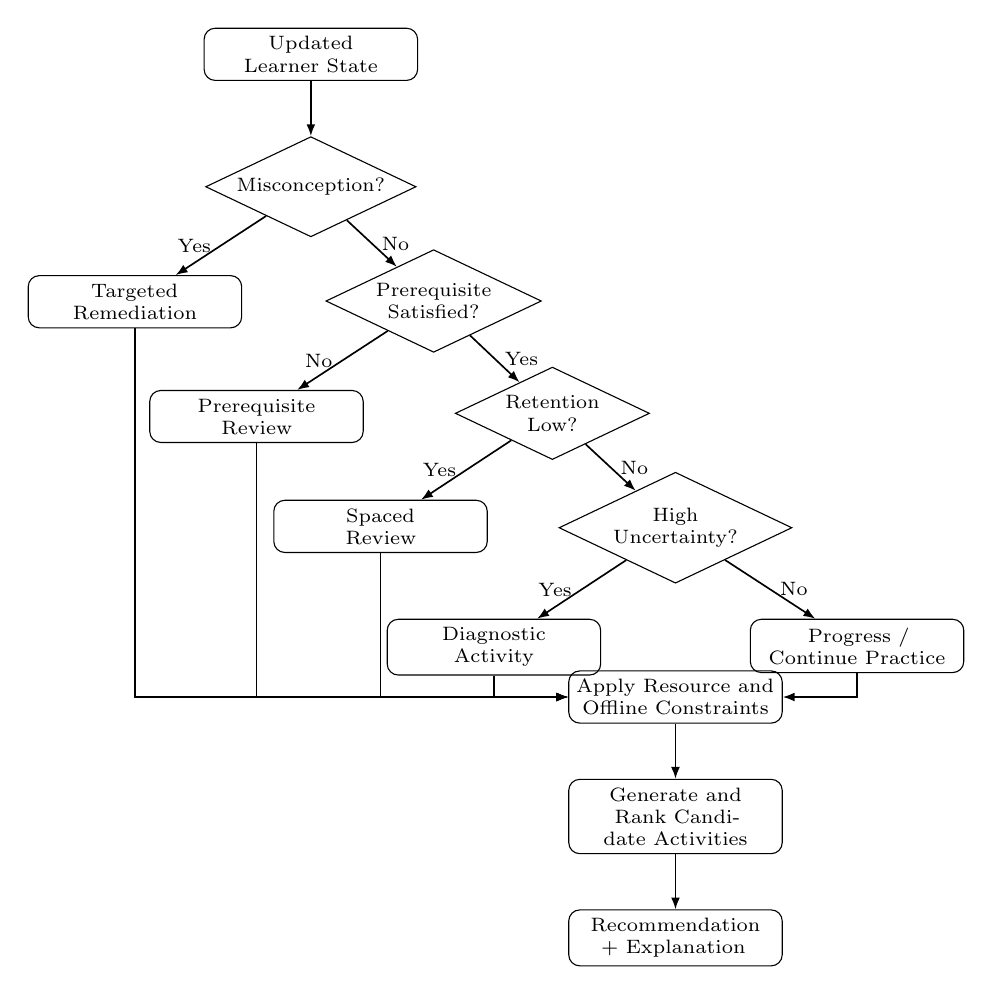
\begin{tikzpicture}[
    node distance=0.7cm,
    every node/.style={font=\scriptsize},
    process/.style={
        rectangle,
        rounded corners,
        draw,
        align=center,
        text width=2.5cm,
        minimum height=0.6cm,
        inner sep=3pt
    },
    decision/.style={
        diamond,
        draw,
        align=center,
        aspect=2.1,
        inner sep=1.5pt
    },
    arrow/.style={-{Latex[length=1.5mm]}, semithick}
]

\node[process] (state) {Updated Learner State};

\node[decision, below=of state] (mis) {Misconception?};

\node[process, below left=0.8cm and 0.2cm of mis] (remed)
{Targeted\\Remediation};

\node[decision, below right=0.8cm and 0.2cm of mis] (pre)
{Prerequisite\\Satisfied?};

\node[process, below left=0.8cm and 0.2cm of pre] (review)
{Prerequisite\\Review};

\node[decision, below right=0.8cm and 0.2cm of pre] (ret)
{Retention\\Low?};

\node[process, below left=0.8cm and 0.2cm of ret] (spaced)
{Spaced\\Review};

\node[decision, below right=0.8cm and 0.2cm of ret] (unc)
{High\\Uncertainty?};

\node[process, below left=0.8cm and 0.2cm of unc] (diag)
{Diagnostic\\Activity};

\node[process, below right=0.8cm and 0.2cm of unc] (progress)
{Progress /\\Continue Practice};

\node[process, below=1.1cm of unc] (resource)
{Apply Resource and Offline Constraints};

\node[process, below=of resource] (rank)
{Generate and Rank Candidate Activities};

\node[process, below=of rank] (output)
{Recommendation + Explanation};

\draw[arrow] (state) -- (mis);

\draw[arrow] (mis) -- node[left]{Yes} (remed);
\draw[arrow] (mis) -- node[right]{No} (pre);

\draw[arrow] (pre) -- node[left]{No} (review);
\draw[arrow] (pre) -- node[right]{Yes} (ret);

\draw[arrow] (ret) -- node[left]{Yes} (spaced);
\draw[arrow] (ret) -- node[right]{No} (unc);

\draw[arrow] (unc) -- node[left]{Yes} (diag);
\draw[arrow] (unc) -- node[right]{No} (progress);

\draw[arrow] (remed) |- (resource);
\draw[arrow] (review) |- (resource);
\draw[arrow] (spaced) |- (resource);
\draw[arrow] (diag) |- (resource);
\draw[arrow] (progress) |- (resource);

\draw[arrow] (resource) -- (rank);
\draw[arrow] (rank) -- (output);

\end{tikzpicture}
}

\caption{Simplified adaptive decision flow used by the RAPID-Learn controller.}
\label{fig:adaptive_flow}
\end{figure}

\subsection{Candidate Activity Generation}

Once an adaptation pathway has been established, the recommendation component identifies eligible learning activities.

Candidate generation considers:

\begin{itemize}
    \item curriculum and subject scope,
    \item activity lifecycle state,
    \item supported adaptation pathway,
    \item prerequisite conditions,
    \item learner history,
    \item misconception compatibility,
    \item offline-content availability, and
    \item computational feasibility.
\end{itemize}

Recently selected activities can be excluded when suitable alternatives exist, reducing unnecessary repetition.

For offline operation, the availability of the application interface alone is not considered sufficient evidence that an instructional activity can be accessed. Candidate resolution verifies actual cached or bundled educational content.

\subsection{Activity Ranking}

Eligible activities are ranked using pedagogical utility and resource cost. The current implementation combines expected learning gain $G$, prerequisite relevance $P$, retention need $R_t$, information gain $I$, misconception relevance $M_c$, and resource-adjusted computational cost $C_r$.

The activity score is expressed as

\begin{equation}
S(a)=0.30G+0.20P+0.20R_t+0.15I+0.10M_c-0.05C_r.
\end{equation}

The weighting emphasizes expected learning benefit while retaining explicit contributions from prerequisites, forgetting, diagnostic value, misconception evidence, and computational feasibility.

Both the resource-score and activity-ranking weights are heuristic design
parameters; they were neither learned nor optimized from learner outcomes. A
separate sensitivity analysis perturbed these weights around their configured
values. Resource-weight variants retained recommendation stability of 1.000,
while the three activity variants retained mean stability of 0.9998, 0.9766,
and 0.9844. Corresponding normalized-gain changes were small, and no tested
perturbation reversed the principal conclusions. These checks assess local
robustness only and do not establish that the chosen weights are optimal.

The distinction between controller pathway selection and candidate ranking is deliberate. The controller determines the pedagogical reason for adaptation, whereas the recommender selects a suitable activity within the resulting constraints.

\subsection{Optional Lightweight Response Prediction}

RAPID-Learn optionally uses logistic regression to predict learner
responses for candidate activities. The model uses learner and activity
features available at recommendation time.

Candidate-specific features can include retained mastery, recent correctness,
activity difficulty, concept difficulty, practice history, elapsed practice
time, prerequisite state, and resource score.

Before ML-based recommendation is enabled, the runtime validates the model artifact, expected artifact version, preprocessing pipeline, feature order, and validation inference. Failure at any of these stages does not prevent adaptation.

Instead, the system performs a complete fallback to BKT-based recommendation and records the reason for the fallback. Partially predicted candidate rankings are not reported.

The machine-learning component is therefore treated as an optional enhancement rather than a dependency of the adaptive architecture.

\subsection{Offline Adaptation}

The learner interface is implemented as a progressive web application. Successfully retrieved instructional activity payloads can be cached locally using IndexedDB.

When connectivity is unavailable:

\begin{itemize}
    \item previously cached learning activities remain accessible;
    \item learner responses are added to a local interaction queue;
    \item available offline activities can continue to support learning; and
    \item queued interactions can be synchronized after connectivity is restored.
\end{itemize}

Educational content is cached separately from the application shell. Therefore, an activity is not considered available offline merely because the interface itself has been cached.

Offline-content availability therefore becomes part of recommendation feasibility rather than being treated solely as a frontend implementation detail.

\section{Experimental Methodology}

The evaluation uses deterministic synthetic learners to examine implementation
behaviour, component contributions, and computational characteristics. It does
not evaluate real students and cannot establish classroom effectiveness. The
simulator maintains latent mastery and misconception state separately from the
RAPID-Learn learner model. Only generated answers, response times, hint use,
and resource observations enter the application pipeline; latent variables and
future responses are unavailable to the controller.

\begin{figure}[t]
\centering
\resizebox{0.92\columnwidth}{!}{%
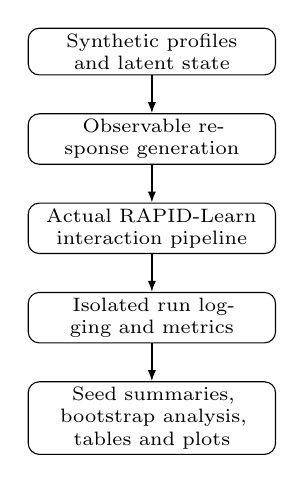
\begin{tikzpicture}[
node distance=0.48cm,
box/.style={rectangle,rounded corners,draw,align=center,text width=3.0cm,
minimum height=0.52cm,inner sep=2pt,font=\scriptsize},
arrow/.style={-{Latex[length=1.4mm]},semithick}]
\node[box] (profiles) {Synthetic profiles and latent state};
\node[box, below=of profiles] (responses) {Observable response generation};
\node[box, below=of responses] (runtime) {Actual RAPID-Learn interaction pipeline};
\node[box, below=of runtime] (logging) {Isolated run logging and metrics};
\node[box, below=of logging] (analysis) {Seed summaries, bootstrap analysis, tables and plots};
\draw[arrow] (profiles) -- (responses);
\draw[arrow] (responses) -- (runtime);
\draw[arrow] (runtime) -- (logging);
\draw[arrow] (logging) -- (analysis);
\end{tikzpicture}}
\caption{Evaluation workflow. Simulator-only latent state generates observable
responses but is not exposed to the adaptive controller.}
\label{fig:evaluation_workflow}
\end{figure}

\subsection{Population and Configuration}

Each primary condition contains 500 learners and 40 interactions per learner.
The nine conditions were executed for seeds 11, 22, 33, 44, and 55, giving 45
isolated condition--seed runs and exactly
$500\times40\times9\times5=900{,}000$ synthetic interactions. Every run used
an isolated in-memory SQLite database. The system learner state began at
mastery 0.20, the mastery threshold was 0.80, and curriculum content came from
the NCERT Class 5 Mathematics pack, version 1.0.0. Where a paired comparison
required it, resource exposure was matched by seed. The eight profiles in
Table~\ref{tab:profiles} were equally weighted. Their parameters are heuristic
simulation assumptions, not estimates derived from real learners.

\begin{table*}[t]
\caption{Synthetic learner profiles used in the certified experiment.}
\label{tab:profiles}
\centering
\scriptsize
\setlength{\tabcolsep}{2.4pt}
\resizebox{\textwidth}{!}{%
\begin{tabular}{lccccccccclc}
\hline
\textbf{Profile} & \textbf{$M_0$} & \textbf{Learn} & \textbf{Guess} &
\textbf{Slip} & \textbf{Speed} & \textbf{Hint} & \textbf{Miscon.} &
\textbf{Forget} & \textbf{Interrupt} & \textbf{Resource} & \textbf{Offline} \\
\hline
Fast learner & .65 & .10 & .08 & .05 & .80 & .10 & .08 & .02 & .03 & High-end & .02 \\
Slow learner & .30 & .04 & .08 & .12 & 1.45 & .25 & .12 & .04 & .08 & Mid-range & .05 \\
Elevated guess & .35 & .07 & .28 & .08 & 1.00 & .15 & .10 & .03 & .05 & Mid-range & .05 \\
Elevated slip & .50 & .07 & .05 & .25 & 1.00 & .15 & .10 & .03 & .05 & Mid-range & .05 \\
Stronger forgetting & .50 & .07 & .08 & .10 & 1.00 & .20 & .10 & .12 & .12 & Mid-range & .08 \\
Misconception prone & .40 & .06 & .08 & .12 & 1.00 & .20 & .55 & .04 & .08 & Mid-range & .08 \\
Intermittent & .45 & .06 & .08 & .10 & 1.10 & .20 & .12 & .06 & .45 & Mixed & .25 \\
Constrained resource & .45 & .06 & .08 & .12 & 1.10 & .25 & .12 & .05 & .15 & Low-end & .35 \\
\hline
\end{tabular}}
\end{table*}

\subsection{Conditions}

Table~\ref{tab:conditions} gives the exact runtime switches. ``Ped.'' denotes
prerequisite and misconception-aware pedagogical rules. Ablations alter the
runtime interaction path, rather than merely relabelling results. The
\texttt{no\_ml} and \texttt{no\_offline\_adaptation} runs are auxiliary
matched-seed controls and are not members of the nine-condition primary suite.

\begin{table*}[t]
\caption{Primary experimental-condition matrix (1 = enabled).}
\label{tab:conditions}
\centering
\scriptsize
\begin{tabular}{lcccccccc}
\hline
\textbf{Condition} & \textbf{BKT} & \textbf{Uncert.} & \textbf{Forget.} &
\textbf{Prereq.} & \textbf{Miscon.} & \textbf{Resource} & \textbf{Offline} & \textbf{ML} \\
\hline
Static & 0&0&0&0&0&0&0&0\\
BKT only & 1&0&0&0&0&0&0&0\\
BKT + uncertainty & 1&1&0&0&0&0&0&0\\
Pedagogical adaptive & 1&1&1&1&1&0&0&0\\
Full RAPID-Learn & 1&1&1&1&1&1&1&1\\
No uncertainty & 1&0&1&1&1&1&1&1\\
No forgetting & 1&1&0&1&1&1&1&1\\
No misconceptions & 1&1&1&1&0&1&1&1\\
No resource awareness & 1&1&1&1&1&0&1&1\\
\hline
\end{tabular}
\end{table*}

\subsection{Metric Definitions}

Accuracy is the mean binary correctness over interactions. Mastery gain is
post-interaction synthetic mastery minus initial synthetic mastery. Synthetic
normalized gain is the concept mean of
\begin{equation}
g=\frac{M_{post}-M_{pre}}{\max(1-M_{pre},10^{-9})}.
\end{equation}
Synthetic retention is
$\min(1,M_{retained}/\max(M,10^{-9}))$. Time to mastery is the first
interaction at which estimated mastery reaches the configured 0.80 threshold;
learners never reaching it are treated as censored for the threshold-time
summary. Conditional on a detected prerequisite gap, a violation occurs when
the system neither selects the prerequisite pathway nor the unmet prerequisite
concept. Misconception resolution requires an exact-ID synthetic intensity to
cross its configured resolved threshold after matching remediation.

For normalized gain $g$, resource-normalized utility is
\begin{equation}
U_R=\frac{g}{1+0.25(L+M_p+C_p+B_w)},
\end{equation}
where $L=\operatorname{clip}(\text{latency}/10\text{ ms})$, $M_p$ is clipped
memory pressure, $C_p$ is clipped CPU fraction, and
$B_w=\operatorname{clip}(\text{bandwidth}/1024\text{ KB})$; all four terms are
bounded to $[0,1]$. Valid offline availability is the fraction of offline
interactions for which the resolver confirms bundled or explicitly cached
educational content; an application shell alone does not qualify. Controller
latency covers pathway selection only, recommendation latency covers
generation, scoring, optional inference, fallback, and selection, and total
adaptive latency covers learner-state processing through prepared
recommendation. All are measured in milliseconds with a monotonic
high-resolution clock. Memory is in MiB, CPU is a percentage, bandwidth is KB
per interaction, and estimated compute cost remains separate from measured
latency.

For temporally matched ML observations, Brier score is
$n^{-1}\sum_i(p_i-y_i)^2$ and log loss is
$-n^{-1}\sum_i[y_i\log p_i+(1-y_i)\log(1-p_i)]$, with probabilities clipped
only for numerical stability. ROC--AUC is the probability that a randomly
selected positive receives a higher score than a randomly selected negative
and is omitted when only one class exists. Calibration is reported from
ten equal-width probability bins as their frequency-weighted absolute
predicted-versus-observed gap; empty bins are ignored. All such
diagnostics concern synthetic outcomes.

\subsection{Statistical Analysis and Reproducibility}

The analysis used 10,000 percentile-bootstrap resamples at 95\% confidence.
For primary condition estimates, the resampling unit was the condition-level
seed summary; for comparisons, it was the matched within-seed Full-minus-
comparison difference. This respects seed-level dependence rather than
resampling individual interaction rows as independent observations.

The frozen configuration, source and analysis Git revisions, configuration
hash, curriculum version, seeds, Python and package versions, timestamps, and
model-artifact version were recorded. Raw CSV and Parquet data, learner and
concept metrics, seed summaries, confidence intervals, paired comparisons,
tables, and figures were validated against the same canonical suite. Every
generated artifact is labelled synthetic.

\section{Synthetic Evaluation Results}

All findings in this section describe the certified synthetic dataset. They are
system-behaviour evidence and not estimates of classroom effectiveness.

\subsection{Overall Adaptive Performance}

Table~\ref{tab:overall_results} reports the primary condition estimates and
seed-level percentile-bootstrap confidence intervals.

\begin{table*}[t]
\caption{Certified synthetic evaluation summary (mean and 95\% CI; values
rounded for display).}
\label{tab:overall_results}
\centering
\scriptsize
\setlength{\tabcolsep}{2.5pt}
\resizebox{\textwidth}{!}{
\begin{tabular}{lccccc}
\hline
\textbf{Condition} &
\textbf{Accuracy} &
\textbf{Normalized Gain} &
\textbf{Retention} &
\textbf{Latency (ms)} &
\textbf{Resource Utility} \\
\hline
Static & .51075 [.50755,.51355] & .30339 [.30193,.30514] & .92216 [.92123,.92319] & 22.167 [21.692,22.547] & .20295 [.20158,.20467]\\
BKT only & .46110 [.45750,.46371] & .19939 [.19754,.20164] & .96188 [.96123,.96253] & 21.926 [21.470,22.383] & .13517 [.13361,.13711]\\
BKT + uncertainty & .46088 [.45679,.46362] & .19950 [.19786,.20176] & .96188 [.96123,.96253] & 21.638 [20.970,22.226] & .13524 [.13382,.13723]\\
Pedagogical adaptive & .55710 [.55488,.55971] & .15252 [.15123,.15354] & .96188 [.96123,.96253] & 22.800 [22.340,23.216] & .10271 [.10168,.10360]\\
Full RAPID-Learn & .55688 [.55477,.55913] & .15229 [.15122,.15333] & .96188 [.96123,.96253] & 22.134 [19.947,23.589] & .10255 [.10165,.10344]\\
No uncertainty & .55722 [.55477,.56020] & .15271 [.15152,.15402] & .96188 [.96123,.96253] & 22.071 [19.674,23.495] & .10279 [.10182,.10390]\\
No forgetting & .55717 [.55442,.56028] & .15213 [.15052,.15380] & .96188 [.96123,.96253] & 24.928 [21.846,26.909] & .10242 [.10109,.10386]\\
No misconceptions & .47649 [.47250,.48157] & .14590 [.14385,.14806] & .96187 [.96122,.96251] & 21.447 [18.461,23.295] & .09953 [.09785,.10135]\\
No resource awareness & .55734 [.55511,.55971] & .15242 [.15141,.15342] & .96188 [.96123,.96253] & 22.775 [20.041,24.439] & .10263 [.10175,.10351]\\
\hline
\end{tabular}
}
\end{table*}

Full RAPID-Learn produced accuracy 0.55688 (95\% CI
[0.55477, 0.559125]) versus 0.51075 [0.50755, 0.51355] for Static, and
retention 0.961882 [0.961232, 0.962526] versus 0.922161
[0.921230, 0.923193]. In contrast, Full normalized gain was 0.152291
[0.151216, 0.153329], substantially below Static at 0.303387
[0.301933, 0.305137]. Full latency was 22.1341~ms
[19.9475, 23.5887], and resource-normalized utility was 0.102545
[0.101647, 0.103443]. Thus, the full controller exhibited higher immediate
accuracy and retention but lower synthetic normalized gain; the evaluation
does not demonstrate general educational superiority.

\begin{figure*}[t]
\centering
\includegraphics[width=0.88\textwidth]{figure_4_normalized_gain.pdf}
\caption{Synthetic normalized gain by primary condition. Error bars are 95\%
percentile-bootstrap confidence intervals over seed-level summaries.}
\label{fig:normalized_gain}
\end{figure*}

\subsection{Component Ablation Analysis}

Misconception handling yielded the clearest positive component result. The
matched Full-minus-No-Misconceptions accuracy difference was +0.080390 (95\%
CI [+0.077240,+0.082540]), and normalized gain differed by +0.006386
[+0.004855,+0.008172]. Removing uncertainty or forgetting produced only small,
mixed changes across the reported measures. The Full-versus-pedagogical-only
difference was likewise small and mixed. These results support a component-
specific interpretation rather than attributing a uniform benefit to every
adaptive mechanism.

\subsection{Resource-Aware Behaviour}

The controller's resource-dependent pathways and cost-sensitive ranking were
exercised, but the matched data did not establish a learning or utility
advantage. Full minus No-Resource-Awareness normalized gain was $-0.000132$
(95\% CI [$-0.000306$,+0.000048]), and the resource-normalized utility
difference was $-0.000087$ [$-0.000205$,+0.000032]. Both intervals include
zero. Figure~\ref{fig:resource_performance} reports the associated resource
comparison without treating these differences as established effects.

\begin{figure*}[t]
\centering
\includegraphics[width=0.88\textwidth]{figure_5_resource_performance.pdf}
\caption{Resource-performance comparison for the certified synthetic suite.
Intervals are 95\% percentile-bootstrap confidence intervals over seed-level
summaries; the figure characterizes simulated system behaviour.}
\label{fig:resource_performance}
\end{figure*}

\subsection{Offline Behaviour}

Validated educational-content availability was 0.2497 (95\% CI
[0.2321,0.2695]). The Full condition selected the cached pathway only 3 times
in 100,000 interactions; across the nine-condition primary suite it appeared
32 times in 900,000 interactions. The auxiliary No-Offline control selected it
zero times. Full minus No-Offline normalized gain was $-0.0000118$
[$-0.0000261$,$-0.0000020$], a statistically directional but practically very
small synthetic difference. Cached-path use was rare, and these checks do not
establish real-world offline deployment success. Application-shell caching was
excluded from educational-content availability.

\subsection{Optional Prediction Model}

The primary suite selected ML 5,216 times among 900,000 interactions; Full
accounted for 362 selections among 100,000 interactions. Of those Full
selections, 344 had a matched subsequent outcome. Mean seed-level Brier score
was 0.6048 (95\% CI [0.5620,0.6289]), indicating poor probability quality in
this synthetic setting. Full minus the auxiliary No-ML control was +0.000160
for accuracy [$-0.000120$,+0.000460] and $-0.000142$ for normalized gain
[$-0.000450$,+0.000153]; neither interval excludes zero. Complete BKT fallback
was verified through fault injection, although no natural fallback occurred in
the accepted Full runs. Consequently, the experiment establishes neither
incremental educational benefit nor satisfactory calibration for the optional
predictor.

\section{Discussion}

\subsection{Accuracy, Retention, and Gain Trade-off}

Under synthetic evaluation, Full RAPID-Learn showed higher response accuracy
and retained mastery than Static but substantially lower normalized gain. The
finding is therefore a trade-off, not general superiority. One interpretation
is that the controller's remediation and review choices supported immediate
success and retention while the Static sequence exposed the simulator to more
opportunities for latent-state growth. Adaptive-learning research similarly
warns that mastery, difficulty, and learning efficiency need not move together
\cite{pelanek2025hard,tan2025}. Because the outcome generator is synthetic,
the trade-off must be tested with real learners before drawing instructional
conclusions.

\subsection{Misconception Handling}

Removing misconception handling caused the largest clear deterioration:
accuracy fell by 0.080390 and normalized gain by 0.006386 relative to Full,
with both paired intervals excluding zero. The exact-ID remediation mechanism
therefore contributed meaningfully within the simulator. This accords with the
broader motivation for interpretable, rule-supported learner modelling
\cite{pelanek2024rules,sajja2025}. The magnitude is conditional on the
heuristic misconception-prone profile and curated rule mappings and should not
be projected onto real students.

\subsection{Uncertainty and Forgetting}

The uncertainty and forgetting ablations produced small or mixed changes.
Their implementations and controller reachability were verified, but the
accepted experiment does not establish a consistent incremental learning
benefit. This may reflect limited synthetic time horizons, interaction between
controller priorities, or simulator assumptions. The result cautions against
equating architectural sophistication with measured benefit.

\subsection{Resource-Aware Behaviour}

The Full-minus-No-Resource-Awareness intervals for normalized gain and
resource-normalized utility both included zero. Thus, although resource
monitoring and resource-sensitive routing functioned as designed, this study
did not establish an outcome advantage. Infrastructure constraints remain a
well-motivated educational concern \cite{hariyanto2025,mimoudi2025,
vandenberg2025}, but the current simulator and exposure mix may be insufficient
to demonstrate the value of this particular policy.

\subsection{Offline Behaviour}

The resolver correctly separated educational content from the application
shell, and the No-Offline control eliminated cached selections. Nevertheless,
the cached pathway was rare: 32 selections in the primary 900,000-interaction
suite. The tiny directional normalized-gain difference is not evidence of a
practically important deployment effect. Field testing under sustained and
realistic connectivity loss remains necessary.

\subsection{Optional Predictor}

The optional logistic-regression model was invoked by the runtime and complete
BKT fallback was verified under injected failures. Its Brier score of 0.6048
showed poor synthetic calibration, and matched Full-minus-No-ML intervals
included zero for both accuracy and normalized gain. These findings support
keeping prediction optional and auditable rather than allowing it to replace
the deterministic pedagogical controller, particularly given concerns about
data dependence in more model-centric approaches \cite{ruan2025,naseer2024,
amin2023}.

\subsection{Weight Sensitivity}

All tested resource-weight variants retained recommendation stability 1.000;
activity-weight variants retained approximately 0.9998, 0.9766, and 0.9844.
Normalized-gain changes remained small, and no tested perturbation reversed the
principal conclusions. This supports local robustness to the specified small
perturbations, but not global optimality of the heuristic weights.

\subsection{Threats to Validity}

\subsubsection{Internal Validity}
The simulator and controller states were tested for separation, and each
condition--seed pair used isolated storage. Even so, synthetic response and
learning transitions are determined by heuristic profile parameters, and
unmodelled interactions among controller rules may influence observed effects.

\subsubsection{Construct Validity}
Accuracy, normalized gain, retained mastery, and resource-normalized utility
are simulation proxies. They do not directly represent understanding,
engagement, or classroom attainment. Curriculum and misconception metadata are
curated prototype assumptions, cached-path execution was rare, and optional ML
probabilities were poorly calibrated against synthetic outcomes.

\subsubsection{External Validity}
All learners and outcomes are synthetic, no classroom or real-student study has
been performed, and the content is limited to NCERT Class 5 Mathematics.
Results may not generalize to other curricula, languages, ages, devices, or
connectivity environments. Full's lower normalized gain than Static and BKT
baselines is an explicit limitation rather than evidence of universal benefit.

\subsubsection{Statistical Conclusion Validity}
Only five independent seeds were available, limiting confidence-interval
resolution despite 10,000 bootstrap resamples. Matched intervals containing
zero were not interpreted as established differences. Latency also depends on
hardware, scheduling, and runtime conditions, so absolute timings are not
universal benchmarks.

\section{Conclusion and Future Work}

RAPID-Learn contributes an auditable adaptive-learning prototype that combines
BKT, independent uncertainty, forgetting, prerequisites, concept-scoped
misconceptions, resource monitoring, offline-content validation, and optional
candidate-level prediction. In 900,000 synthetic interactions, Full produced
higher accuracy and retention than Static but substantially lower normalized
gain, so the results do not support overall superiority. Misconception handling
showed the clearest positive ablation effect. Resource awareness did not
establish an incremental gain or utility advantage, while cached-path use was
rare. The optional predictor was poorly calibrated and showed no established
incremental benefit, although full BKT fallback remained reliable. Small
weight perturbations did not reverse these conclusions.

These results validate reproducible controller and system behaviour, not
educational effectiveness. Future work should estimate learner-model and
profile parameters from authentic data, validate misconception mappings with
educators, improve or remove the optional predictor based on real calibration,
and test offline and resource policies on representative devices and networks.
Controlled studies with real learners are necessary before making claims about
learning outcomes, engagement, or classroom usefulness.

\begin{thebibliography}{99}

\bibitem{mittal2024}
U. Mittal, S. Sai, V. Chamola, and D. Sangwan,
``A comprehensive review on generative AI for education,'' 2024.

\bibitem{ruan2025}
S. Ruan and K. Lu,
``Adaptive deep reinforcement learning for personalized learning pathways:
A multimodal data-driven approach with real-time feedback optimization,''
2025.

\bibitem{tan2025}
L. Y. Tan, S. Hu, D. J. Yeo, and K. H. Cheong,
``Artificial intelligence-enabled adaptive learning platforms: A review,''
2025.

\bibitem{pelanek2025hard}
R. Pelánek,
``Adaptive learning is hard: Challenges, nuances, and trade-offs in modeling,''
2025.

\bibitem{dhananjaya2024}
G. M. Dhananjaya, R. H. Goudar, A. A. Kulkarni, V. N. Rathod,
and G. S. Hukkeri,
``A digital recommendation system for personalized learning to enhance
online education: A review,'' 2024.

\bibitem{farhah2025}
N. Farhah, M. Adnan, A. A. Alqarni, M. I. Uddin,
and T. H. H. Aldhyani,
``AI-driven innovation using multimodal and personalized adaptive education
for students with special needs,'' 2025.

\bibitem{hariyanto2025}
Hariyanto, F. X. D. Kristianingsih, and R. Maharani,
``Artificial intelligence in adaptive education: A systematic review of
techniques for personalized learning,'' 2025.

\bibitem{ifenthaler2024}
D. Ifenthaler, R. Majumdar, P. Gorissen, M. Judge, S. Mishra,
J. Raffaghelli, and A. Shimada,
``Artificial intelligence in education: Implications for policymakers,
researchers, and practitioners,'' 2024.

\bibitem{pereira2025}
A. F. Pereira and R. F. Mello,
``A systematic literature review on large language models applications in
computer programming teaching evaluation process,'' 2025.

\bibitem{matos2025}
T. Matos, W. Santos, E. Zdravevski, P. J. Coelho, I. M. Pires,
and F. Madeira,
``A systematic review of artificial intelligence applications in education:
Emerging trends and challenges,'' 2025.

\bibitem{mejeh2025codesign}
M. Mejeh and L. Sarbach,
``Co-design: From understanding to prototyping an adaptive learning
technology to enhance self-regulated learning,'' 2025.

\bibitem{tzirides2024}
A. O. Tzirides, G. Zapata, N. P. Kastania, A. K. Saini, V. Castro,
S. A. Ismael, Y.-L. You, T. A. dos Santos, D. Searsmith,
C. O'Brien, B. Cope, and M. Kalantzis,
``Combining human and artificial intelligence for enhanced AI literacy
in higher education,'' 2024.

\bibitem{boltsi2024}
A. Boltsi, K. Kalovrektis, A. Xenakis, P. Chatzimisios,
and C. Chaikalis,
``Digital tools, technologies, and learning methodologies for Education 4.0
frameworks: A STEM oriented survey,'' 2024.

\bibitem{dai2024}
Y. Dai, H. U. Hoppe, B. Flanagan, K. Takami, and H. Ogata,
``Do personal recommendations need to be personalized? Investigating the
relationships between student differences and educational recommendations,''
2024.

\bibitem{ezzaim2024}
E. Aymane, D. Aziz, H. Abdelfatteh, and A. Abdelhak,
``Enabling sustainable learning: A machine learning approach for an
eco-friendly multi-factor adaptive e-learning system,'' 2024.

\bibitem{pahi2024}
K. Pahi, S. Hawlader, E. Hicks, A. Zaman, and V. Phan,
``Enhancing active learning through collaboration between human teachers
and generative AI,'' 2024.

\bibitem{li2025}
J. Li,
``Enhancing learning through an adaptive web-based educational search
framework integrating natural language processing and machine learning
techniques,'' 2025.

\bibitem{fujii2024}
A. Fujii,
``Exploring autonomy support and learning preference in higher education:
Introducing a flexible and personalized learning environment with
technology,'' 2024.

\bibitem{samat2026}
C. Samat, P. Kwangmuang, P. Vongtathum, I. Kanjug, T. Wannasen,
P. Duangngern, N. Gessala, P. Sarakan, R. Pitakaso, and T. T. Wu,
``Generative AI for adaptive curriculum design enhances student performance
and engagement in technology-enhanced learning environments,'' 2026.

\bibitem{tasdelen2025}
O. Tasdelen and D. Bodemer,
``Generative AI in the classroom: Effects of context-personalized learning
material and tasks on motivation and performance,'' 2025.

\bibitem{mimoudi2025}
A. Mimoudi,
``Generative AI to bridge the educational divide: Personalized learning
and challenges,'' 2025.

\bibitem{hassanain2025}
A. A. Hassanain, Y. Amor, R. Abidi, and N. Sahli,
``Impact of machine learning on personalized learning and course
customization,'' 2025.

\bibitem{sajja2025}
R. Sajja, Y. Sermet, D. Cwiertny, and I. Demir,
``Integrating AI and learning analytics for data-driven pedagogical
decisions and personalized interventions in education,'' 2025.

\bibitem{naseer2024}
F. Naseer, M. N. Khan, M. Tahir, A. Addas, and S. M. H. Aejaz,
``Integrating deep learning techniques for personalized learning pathways
in higher education,'' 2024.

\bibitem{halkiopoulos2024}
C. Halkiopoulos and E. Gkintoni,
``Leveraging AI in e-learning: Personalized learning and adaptive
assessment through cognitive neuropsychology,'' 2024.

\bibitem{duplooy2024}
E. du Plooy, D. Casteleijn, and D. Franzsen,
``Personalized adaptive learning in higher education: A scoping review of
key characteristics and impact on academic performance and engagement,''
2024.

\bibitem{denden2025}
M. Denden and M. Abed,
``Personalized learning policies and strategies in K--12 education:
Where, when, and for what?'' 2025.

\bibitem{gunawardena2024}
M. Gunawardena, P. Bishop, and K. Aviruppola,
``Personalized learning: The simple, the complicated, the complex and
the chaotic,'' 2024.

\bibitem{pelanek2024rules}
R. Pelánek, T. Effenberger, and P. Jarušek,
``Personalized recommendations for learning activities in online
environments: A modular rule-based approach,'' 2024.

\bibitem{amin2023}
S. Amin, M. I. Uddin, A. A. Alarood, W. K. Mashwani,
A. Alzahrani, and A. O. Alzahrani,
``Smart e-learning framework for personalized adaptive learning and
sequential path recommendations using reinforcement learning,'' 2023.

\bibitem{jin2023}
S.-H. Jin, K. Im, M. Yoo, I. Roll, and K. Seo,
``Supporting students' self-regulated learning in online learning using
artificial intelligence applications,'' 2023.

\bibitem{mejehrehm2024}
M. Mejeh and M. Rehm,
``Taking adaptive learning in educational settings to the next level:
Leveraging natural language processing for improved personalization,''
2024.

\bibitem{lee2024}
S. Lee and K.-S. Song,
``Teachers' and students' perceptions of AI-generated concept explanations:
Implications for integrating generative AI in computer science education,''
2024.

\bibitem{vandenberg2025}
G. van den Berg,
``Teachers' experiences of using artificial intelligence from an open
distance learning context: Successes, challenges, and strategies for
success,'' 2025.

\bibitem{chen2025}
D.-L. Chen, K. Aaltonen, H. Lampela, and J. Kujala,
``The design and implementation of an educational chatbot with personalized
adaptive learning features for project management training,'' 2025.

\bibitem{merino2025}
C. Merino-Campos,
``The impact of artificial intelligence on personalized learning in higher
education: A systematic review,'' 2025.

\bibitem{contrino2024}
M. F. Contrino, M. Reyes-Millán, P. Vázquez-Villegas,
and J. Membrillo-Hernández,
``Using an adaptive learning tool to improve student performance and
satisfaction in online and face-to-face education for a more personalized
approach,'' 2024.

\end{thebibliography}

\end{document}
